\documentclass[12pt,a4paper]{article}
%\usepackage{a4, indentfirst}
\usepackage[utf8]{inputenc}
\usepackage[czech]{babel}
\usepackage{color}
\usepackage[dvipsnames]{xcolor}
\usepackage[T1]{fontenc}
\usepackage{tikz}
\usepackage{filecontents}
\usepackage{graphicx}
\usepackage{amsfonts}
\usepackage{amsthm}
\usepackage{listings}
\usepackage{tabularx}
\newtheorem{theorem}{Theorem}
\usepackage[font=footnotesize]{subcaption}
\usepackage[colorlinks]{hyperref}
\hypersetup{citecolor=black}
\hypersetup{linkcolor=black}
\hypersetup{urlcolor=blue}
\usepackage{rotating}

\title{\LaTeX{} - DIPR}
\date{December 2016}
\author{N1915H}

\begin{document}
	\maketitle
	\newpage
	\section*{Předmluva}
	Zápočet bude udělen za vypracování následujících úkolů.
\begin{itemize} \itemsep-2pt \rightskip-5pt
	\item požadováno vypracování zápočtového dokumentu v LaTeXu s obrázkem v METAPOSTu nebo TikZu a komentáře k závěrečné práci
	\item požadavky na zápočtový dokument v LaTeXu: výstup do PDF, český text (diakritika, uvozovky), změna vlastnosti písma (sf, bf, it, velikost), zdrojový\linebreak text z programovacího jazyka, seznam, tabulka (čáry mezi buňkami,\linebreak sloučené buňky), matematika (vzorec, rovnice, matice, věta, důkaz), sekce a odkazy na ně, obsah, vložený obrázek s odkazem na něj, seznam literatury\linebreak ručně nebo v BibTeXu, citace do seznamu v textu, barevný text, hypertextový odkaz v PDF
	\item požadavky na obrázek v METAPOSTu nebo TikZu: výstup do PDF,\linebreak lomená čára nebo křivka (např. obdélník, kružnice), transformace, barva, oříznutí, vyplnění nebo cyklus, text v LaTeXu, např. graf funkce s osami souřadnic, graf s vrcholy s popisky, diagram s vyplněnými objekty
	\item požadavky na komentář k závěrečné práci: zdůvodněné okomentování\linebreak vybrané závěrečné práce odevzdané na katedře informatiky UP v\linebreak Olomouci (co je dobře a špatně a proč), např. styl v LaTeXu, struktura textu ((TA)IMRaD) a CD/DVD, anotace, poděkování, obrázky (formát), závěry, reference (forma, úplnost, citace), typografie, gramatika, odborný styl (problém, řešení, výsledky, závěry), jazyk. Očekávaný rozsah cca 1 strana v A4, vypracování v LaTeXu.
\end{itemize}
	\newpage
	\tableofcontents
	\pagenumbering{arabic}
	\setcounter{page}{3}
	\newpage
\section{Introduction}{\setcounter{section}{1}}
	\subsection{(RED)}
	\label{red}
	\fontfamily{cmss}\selectfont
	{Naše partnerství s organizací \uv{\textcolor{red}{(RED)}}{\footnote{\url{http://www.apple.com/cz/product-red}} už 10 let pomáhá bojovat proti šíření AIDS zajišťováním poradenství, testování a především léků, které brání přenosu HIV z matky na nenarozené dítě. Každým nákupem se dostáváme o krok blíž ke generaci bez AIDS. Připoj se k našemu úsilí.}
\begin{center}
	\vspace*{0.5cm}
	\textcolor{Maroon} {\huge \uv {Každým nákupem produktu (RED)\linebreak
	příspíváš přímo globálním\linebreak
	fondu na boj proti AIDS.}}
	\vspace*{0.5cm}
	{\color{BrickRed} \rule{\linewidth}{0.3mm}}
	\textcolor{Maroon}{\huge \uv {Jeden dolar zajistí\linebreak třídenní zásobu\linebreak životně důležítých léku.}}
	\vspace*{0.5cm}
	{\color{BrickRed} \rule{\linewidth}{0.3mm}}
	\textcolor{Maroon}{\huge \uv {Tvoje příspěvky financují\linebreak poradenství, vzdělávání\linebreak a péčí o pacienty s HIV}}
	{\color{BrickRed} \rule{\linewidth}{0.3mm}}
	\mbox{\resizebox{15cm}{!}{{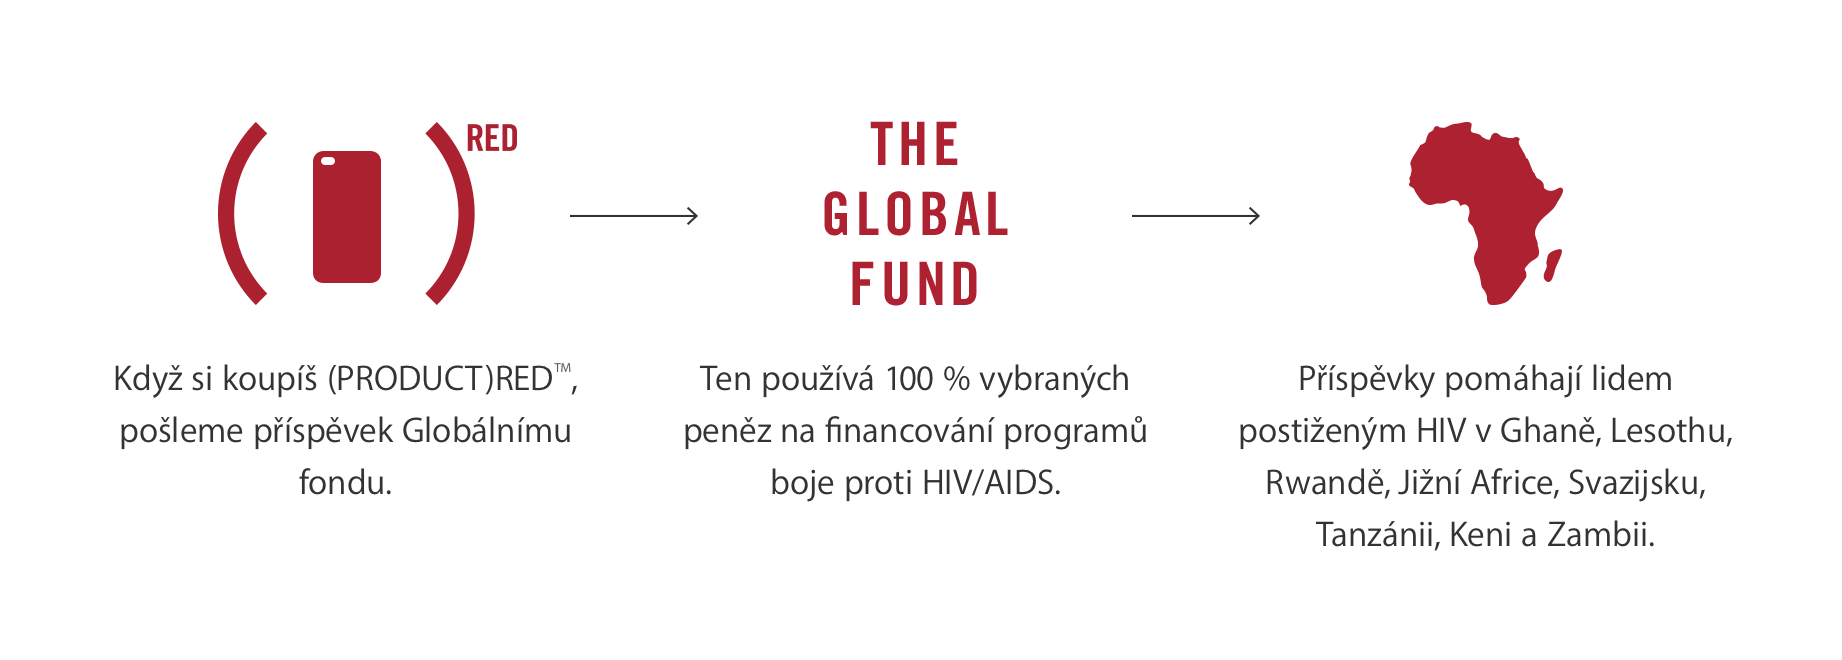
\includegraphics{SN_1.png}}}}
\end{center}
	\newpage
	\subsection{Product RED}
	\label{productred}
	styled as \textcolor{red}{(PRODUCT)\textsuperscript{RED}}, is a licensed brand that seeks to engage the private sector in raising awareness and funds to help eliminate HIV/AIDS in Africa.\\
	\\
	It is licensed to partner companies including \textbf{Nike, American Express (UK), Apple Inc., The Coca-Cola Company, Starbucks, Converse, Electronic Arts, Head, Bugaboo, Penguin Classics (UK and International), Gap, Armani, Hallmark (US), SAP and Beats Electronics (Beats by Dr. Dre), and Supercell.} The concept was founded in 2006 by U2 frontman and activist, Bono, together with Bobby Shriver of the ONE/DATA. The Global Fund to Fight AIDS, Tuberculosis and Malaria is a recipient of (RED) money.\\
	\\
	\textsc{\uv{Product Red}} has been criticized for not having an effect proportional to the advertising investment, for being much less efficient than direct charitable contribution, and for having a lack of transparency with regards to the amount of money going to charity as a percentage of every purchase. Some critics argue that a retail middleman between donor and charity is unnecessary; donors should just give. \texttt{\uv{Like with the Gap website and Campaign Red}}, some argued that it encouraged consumption of the products, thus, encouraging companies to use the product for publicity, rather than social responsibility. Scholars argue that this sacrifices the purpose of movements such as Product Red. Jessica Wirgau, professor at the Virginia Politechnic institute stated that, \textsf{"Red not only misses the opportunity to promote civic engagement with its audience but also.... gives corporations the power to decide which causes should be supported and to what degree".} In the Stanford Social Innovation Review, Mark Rosenman wrote that it was an \textit {"example of the corporate world aligning its operations with its central purpose of increasing shareholder profit, except this time it is being cloaked in the patina of philanthropy."}\\
	\\
	{\tiny {\uv{\textcolor{red}{(N1915H)\textsuperscript{RED}}}}}\\
	\\
	{\large {\uv{\textcolor{red}{(PRODUCT)\textsuperscript{RED}}}}}\\
	\\
	{\huge {\uv{\textcolor{red}{(PRODUCT)\textsuperscript{RED}}}}}
	{\footnote{\url{https://en.wikipedia.org/wiki/Product_Red}}
	\\
	or
	\\
	\url{https://en.wikipedia.org/wiki/Product_Red}
	\newpage
	\section{Coder}
	\subsection{Swift}
	\label{swift}
	Examples:
\begin{lstlisting}
Swift 2.2
	let blue = UIColor.blueColor()
	let min = numbers.minElement()
	attributedString.appendAttributedString(anotherString)
	names.insert("Jane", atIndex: 0)
	UIDevice.currentDevice()
	
Swift 3
	let blue = UIColor.blue
	let min = numbers.min()
	attributedString.append(anotherString)
	names.insert("Jane", at: 0)
	UIDevice.current
\end{lstlisting}
	Can you identify the needless words? When you're working with UIColor, of course blue is going to be a color, so saying {\textcolor{blue} {blueColor()}} is needless. When you append one attributed string to another, do you really need to specify that it's an attributed string you're appending as opposed to an elephant? And why should it be a method – surely a color should be a property!
	\newpage
	\subsection{Shortly about Swift}
	\label{shortlyaboutswift}
\begin{itemize}
	\item Open Source
	\begin{itemize}
	\item Swift 3 is the first major release developed in the open at Swift.org, with source code, a bug tracker, mailing lists, and regular development builds available for everyone.
	\end{itemize}
	\item Refined API Naming
	\begin{itemize}
	\item The syntax and patterns used in popular Swift libraries have almost as much impact on the character of Swift code as the specification of the language itself.
	\end{itemize}
	\item Modern
	\begin{itemize}
	\item Swift is the result of the latest research on programming languages, combined with decades of experience building Apple platforms.
	\end{itemize}
	\item Playgrounds and REPL in Xcode
	\begin{itemize}
	\item Much like Swift Playgrounds for iPad, playgrounds in Xcode make writing Swift code incredibly simple and fun. Type a line of code and the result appears immediately.
	\end{itemize}
	\item Designed for Safety
	\begin{itemize}
	\item Swift eliminates entire classes of unsafe code. Variables are always initialized before use, arrays and integers are checked for overflow, and memory is managed automatically. 
	\end{itemize}
	\item Fast and Powerful
	\begin{itemize}
	\item From its earliest conception, Swift was built to be fast. Using the incredibly high-performance LLVM compiler, Swift code is transformed into optimized native code that gets the most out of modern hardware.
	\end{itemize}
	\item Objective-C Interoperability
	\begin{itemize}
	\item You can create an entirely new application with Swift today, or begin using Swift code to implement new features and functionality in your app.
	\end{itemize}
\end{itemize}
	\newpage
	\section{Table}
	\subsection{L337}
	\label{l337}
	\begin{table}[h!]
	\centering
    \begin{tabular}{|l*{7}{|l}|}
    \hline
    \multicolumn{2}{|l|}{Name n' Surename} & \multicolumn{6}{|c|}{1337} \\ \hline
    \multicolumn{2}{|l|}{Viet T.H.} & N & 1 & 9 & 1 & 5 & H \\
    \hline  
    \end{tabular}  
	\end{table}
	\subsection{Destroyer Class}
	\label{desclass}
	\begin{table}[h!]
	\centering
	\begin{tabular}{|l|l|l|}
 	\hline
 	\multicolumn{1}{|c|}{
    \begin{sideways}
       Empire Destroyer \,
    \end{sideways}}&
       \multicolumn{1}{c|}{
          \begin{sideways}
             Federation Destroyer \,
          \end{sideways}}&
             \multicolumn{1}{c|}{
                \begin{sideways}
                   Jericho Destroyer \,
                \end{sideways}} \\\hline
 	VIII Invinciblea & VIII Procyon & VIII Archon \\\hline
 	XI Brave & XI Antares & XI Sibyl \\\hline
 	XIV Vigilant & XIV Sirius & XIV Tyrant \\\hline
 	\end{tabular}
	\end{table}	
	\newpage	
	\section{Math is universal language}
	\subsection{Vzorec}
	\label{vzorec}
	\begin{displaymath}
	\lim_{n \to \infty}
	\sum_{k=1}^n \frac{1}{k^2}
	= \frac{\pi^2}{6}
	\end{displaymath}
	
	\subsection{Rovnice}
	\label{rovnice}
	\begin{displaymath}
	\frac {k^2(x-1)}{kx-2} = 2 
	\end{displaymath}
	
	\subsection{Matice}
	\label{matice}
	$$5* \left(
	\begin{array}{ccc@{\ }r}
    a & b & c \\
    b & 1 & 2 \\
    c & 1 & 2 \\
    \end{array}
    \right) + 
    \left(
	\begin{array}{ccc@{\ }r}
    c & b & a \\
    b & 2 & 1 \\
    a & 2 & 1 \\
    \end{array}
    \right)$$
    
    \subsection{Důkaz}
    \label{dukaz}
    \begin{proof}
	Zde je důkaz, že platí 
	$(a+b)^{2}$
	\[
	(a+b)*(a+b) = a*a+a*b+b*a+b*b =
	\]
	\[
	= a*a+2ab+b*b = a^2+2ab+b^2
	\]
	\end{proof}
	
	\subsection{Věta}
	\label{veta}
	\begin{theorem}[Pythagorean theorem]
	\label{pythagorean}
	This is a theorema about right triangles and can be summarised in the next equation 
	\[ x^2 + y^2 = z^2 \]
	\end{theorem}
	\newpage
	\section{METAPOST 'n Tikz}
	\subsection{Tikz}
	\label{tikz}
\begin{figure}[h]
    \centering
    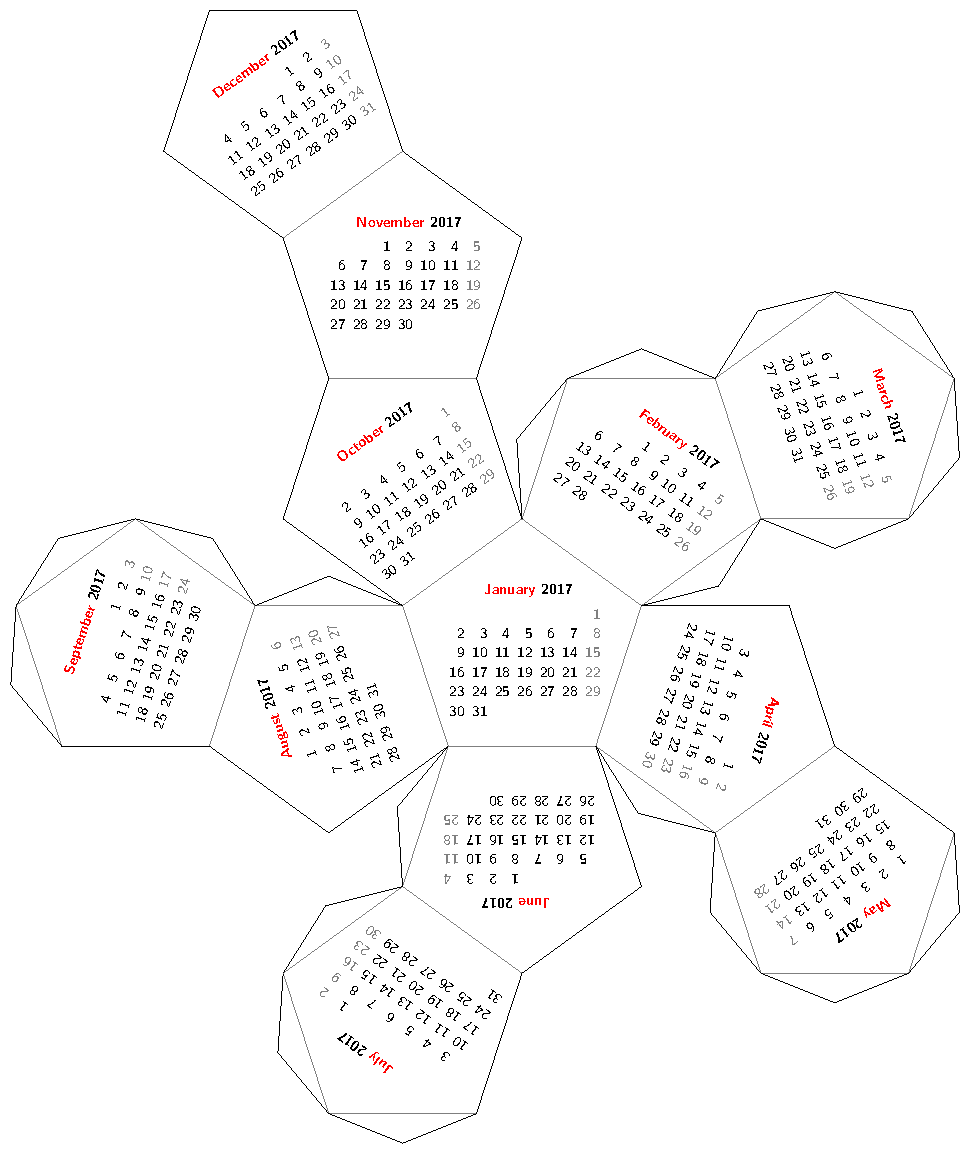
\includegraphics[width=0.93\textwidth]{Tikz}
    \caption{Cal for 2017 (Origami)}
    \label{fig:graf}
\end{figure}
	
	\newpage
	\subsection{Metapost}
	\label{metapost}
	\vspace*{1.5cm}
\begin{figure}[h]
    \centering
    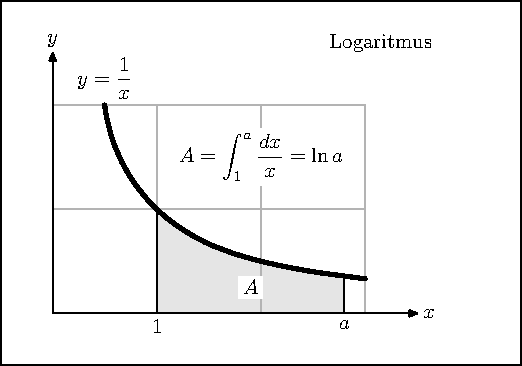
\includegraphics[width=0.99\textwidth]{METAPOST_1-1}
    \caption{Logaritmus}
    \label{fig:graf}
\end{figure}
	\vspace*{1.5cm}
\begin{figure}[h]
    \centering
    
\includegraphics[width=0.55\textwidth]{METAPOST_2-49}
    \caption{Úhel}
    \label{fig:graf}
\end{figure}
	\vspace*{1.5cm}
	\newpage
	\section{Web - hyp3rl1nk}
	\subsection{My FAV. stuff}
	\begin{itemize}
		\item My fav. Japanese song: \url{https://www.youtube.com/watch?v=mHsmyYPqa1M}
		\item \href{https://www.youtube.com/watch?v=vMNFU_6hBfI}{Special Others - Uncle John (JPN)}
		\item My fav Game: \url{http://star-conflict.com}
		\item \href{https://www.youtube.com/watch?v=L2t714QggGc}{Star Conflict - Czech Ravagers [CzR] (Short video)}
	\end{itemize}
	\newpage
	\section{Rejstřík}
	\subsection{First part}
	Red(\ref{red})\\
	Product RED(\ref{productred})
	\subsection{Second part}
	Swift(\ref{swift})\\
	Shortly about Swift(\ref{shortlyaboutswift})
	\subsection{Third part}
	L337(\ref{l337})\\
	Destroyer Class(\ref{desclass})
	\subsection{Four part}
	Vzorec(\ref{vzorec})\\
	Rovnice(\ref{rovnice})\\
	Matice(\ref{matice})\\
	Důkaz(\ref{dukaz})\\
	Věta(\ref{veta})
	\subsection{Fifth part}
	Tikz(\ref{tikz})\\
	Metapost(\ref{metapost})
	\newpage
	\section{List of Literature}
\begin{thebibliography}{9}
	\bibitem{odkaz} RYBIČKA, Jiří.
	\emph{\LaTeX{} pro začátečníky}. 3. vydání.
Brno: Konvoj, 2003. 
ISBN 80-7302-049-1.
	\bibitem{odkaz} Tuja Máximo 
	\emph{Latex for Fun (anglicky)}
Die Gestalten Verlag (DGV), 2007.
ISBN: 978-3-89955-190-7.
	\bibitem{odkaz} Gratzer, George A.
	\emph{Practical LaTeX}
Springer International Publishing AG. 2014
ISBN / EAN 9783319064246 / 9783319064246.
\end{thebibliography}
\end{document}